\begin{figure*}[!t]
    \centering
    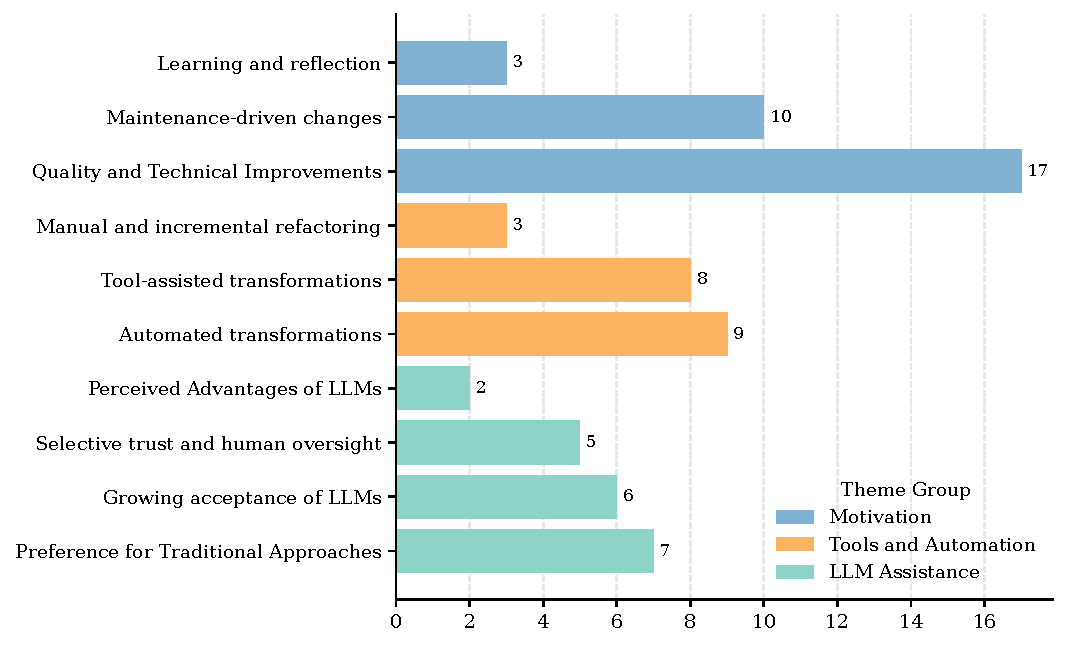
\includegraphics[width=\textwidth]{imgs/rqs_ta.pdf}
\caption{Themes identified from developers' feedback across the three research questions. The numbers represent the frequency of quotations assigned to each theme.}
    \label{fig:motivation_distribution}
\end{figure*}

% This section presents the results of the qualitative investigation conducted to understand the motivations associated with large-scale Type Hint modernization. We first provide an overview of the survey responses obtained from developers responsible for the selected modernization commits, highlighting the main observations. We then present the thematic analysis of the developers feedback, organized according to the three research questions concerning (RQ1) the motivations behind the code changes, (RQ2) the tools and practices employed during the modernization process, and (RQ3) developers perceptions regarding the use of Foundation Models for these tasks. Next, we analyze the corresponding repository artifacts, including commit messages and pull request discussions, to characterize how these motivations and practices are documented in software repositories. Finally, we triangulate both sources of evidence to assess their consistency and identify complementary insights into developers decision-making processes.

\subsection{Overview of Developer Survey Results}

We contacted developers responsible for large-scale modernization commits and then manually validating the candidate commits, we sent 117 emails to developers associated with the recent transformations (2024-2026), while 10 developers were not reachable. Resulting in 107 developers successfully contacted and 20 responses received.

%\todo[inline]{Pessoal, a gente não focou em motivações no estudo anterior. Esse é o foco deste estudo. Alana, pode confirmar isso? Eu lembro de vocês terem olhado os commits / PRs, mas não submetemos tais resultados no paper. Estamos perdendo uma oportunidade aqui neste artigo. E se este trabalho apenas confirma resultados anteriores, ele deixa de ser importante. Eu acho que poderíamos inclusive começar com as análises de Commits / PRs, e usar o survey para complementar as respostas. Como essas mudanças são mais críticas, talvez seja melhor submeter para https://vemworkshop.github.io/vem2026/callForPapers.html. Outra coisa, não estamos evidências que suportam os findings desses parágrafos. Precisamos incluir quotes, links para commits, PRs, etc. Outra opção: https://sbqs.sbc.org.br/2026/index.php/pt/chamada-de-trabalhos/trilha-de-trabalhos-tecnicos}

The reported motivations largely confirm the patterns observed in the mining study. Most developers described the changes as modernization or maintenance activities driven by the evolution of the Python ecosystem, adoption of newer language features, improved readability, better documentation, and stronger static analysis support (\textsc{FastAPI} project -- commit \texttt{3da206c},
\textsc{aiohttp} project -- commit \texttt{35754d4},
\textsc{Wagtail} project -- commit \texttt{80b1ebe})

This is reflected in statements such as:
\begin{quote}
\textit{``Better readability and more expressive code was the main motivation for this change.''} (\textsc{Wagtail} project, commit \texttt{80b1ebe})
\end{quote}

and

\begin{quote}
\textit{``The motivation was due to the deprecation of Python 3.9.''} (\textsc{FastAPI} project, commit \texttt{3da206c})
\end{quote}

Several respondents also highlighted defect prevention and long-term maintainability as important benefits of Type Hints (\textsc{Chia Blockchain} project, commit \texttt{a447734}, \textsc{django-cms} project, commit \texttt{1efaa98}, \textsc{AutoGPT} project, commit \texttt{e16e69c}). For instance:
\begin{quote}
\textit{``This makes the code more resilient against bugs.''} (\textsc{Chia Blockchain} project, commit \texttt{a447734})
\end{quote}

Automation played a central role in many modernization efforts. Developers frequently reported using tools such as \texttt{pyupgrade}, \texttt{ruff}, \texttt{mypy}, and IDE-assisted search-and-replace mechanisms to perform repetitive changes (\textsc{Tornado} project, commit \texttt{113cf79}, \textsc{PyTorch Vision} project, commit \texttt{a095de1}, \textsc{mypy} project, commit \texttt{6682563}).

This is supported by statements such as:
\begin{quote}
\textit{``This commit was generated as part of automated transformations using pyupgrade.''} (\textsc{Tornado} project, commit \texttt{113cf79})
\end{quote}

However, nearly all respondents emphasized the need for manual inspection after automated transformations, particularly in large-scale commits, due to concerns about incorrect modifications and unintended side effects (\textsc{CVAT} project, commit \texttt{5ddeda3}, \textsc{freqtrade} project, commit \texttt{f369151}).

Opinions regarding Foundation Models were more diverse. Some developers viewed LLMs as potentially useful for repetitive typing-related tasks and reported positive experiences using them for code transformations (\textsc{Deep Agents} project, commit \texttt{d398a1e}, \textsc{Pipecat} project, commit \texttt{c4dbe92}). For example:
\begin{quote}
\textit{``Virtually everyone is using agents / LLMs these days for coding.''} (\textsc{Deep Agents} project, commit \texttt{d398a1e})
\end{quote}

and
\begin{quote}
\textit{``Claude Code did almost everything right, but I had to manually edit a few things.''} (\textsc{Pipecat} project, commit \texttt{c4dbe92})
\end{quote}

Others expressed concerns about reliability, predictability, and loss of control over generated changes, preferring deterministic tools for large-scale refactoring activities (\textsc{Wagtail} project, commit \texttt{80b1ebe}, \textsc{Locust} project, commit \texttt{9341cf9}, \textsc{Scrapy} project, commit \texttt{6ecc9e0}).

Finally, the responses are consistent with an important finding from our quantitative analysis: although many Type Hint transformations are mechanical and highly automatable, successful modernization still depends on developer supervision and project-specific decisions (\textsc{Manim} project, commit \texttt{8773252}).

% \todo[inline, color = green]{Essa Seção 5.1 parece mais um resumo dos achados. Uma opção é indicarmos no título da seção que aqui apresentamos apenas um overview das respostas.}

\subsection{Thematic Analysis of Developer Responses}

% \todo[inline, color=green]{TODO: Adicionar hashs dos commits citados}
% \todo[inline, color=green]{TODO: Retirar nome dos autores}
%\todo[inline]{Verificar qual melhor formato para os quotes}
% \todo[inline]{TODO: Adicionar informações, por exemplo, quantas transformações existiam no commit que motivou o contato com o dev.}


\subsubsection{Motivations for Code Changes}
The thematic analysis revealed that large-scale type-related transformations were primarily motivated by quality and technical improvements ($n = 17$). Developers frequently associated these changes with the adoption of modern Python practices, improved readability and maintainability, better IDE support, enhanced static analysis capabilities, and the prevention of subtle bugs. Other responses emphasized architectural concerns, such as reducing code duplication, introducing type abstractions, and addressing limitations in legacy designs. For example, a developer from the \textsc{Wagtail} project (commit ~\texttt{80b1ebe}) explained that adopting newer language features:

\begin{quote}
\textit{``would make the code more readable and expressive''} (\textsc{Wagtail} project, commit ~\texttt{80b1ebe}).
\end{quote}

while a contributor to (\textsc{Chia Blockchain} project, commit ~\texttt{a447734}) noted that the changes were intended to make the code:

\begin{quote}
\textit{``more resilient against bugs''} ( \textsc{Chia Blockchain}, commit ~\texttt{a447734}).
\end{quote}
Maintenance-driven changes represented the second most common motivation theme ($n = 10$). These responses were predominantly associated with the evolution of the Python ecosystem, including the discontinuation of support for older Python versions and dependency maintenance requirements. One respondent from the \textsc{PyTorch Vision} project (commit ~\texttt{a095de1}) explicitly stated that the change was motivated by:

\begin{quote}
\textit{``the motivation was due to the deprecation of Python 3.9.''} (\textsc{PyTorch Vision} project, commit ~\texttt{a095de1})
\end{quote}

whereas another contributor described the modifications as routine maintenance activities. In some cases, ecosystem pressures and quality concerns appeared simultaneously. For instance, a developer from the \textsc{Wagtail} project (commit ~\texttt{80b1ebe}) reported that support for Python 3.8 was being dropped due to its end-of-life status, while newer language features were adopted to improve code quality.

Finally, a small number of responses highlighted learning and reflection as motivations for modernization efforts ($n = 3$). Developers described these transformations as opportunities to gain familiarity with the codebase, improve their understanding of Python typing, and reflect on previous design decisions. 
A developer from the \textsc{Manim} project (commit ~\texttt{8773252}) noted that:
\begin{quote}
\textit{``Adding type annotations allowed me to learn about the source code ... improve my skills related type annotations in python.''} (\textsc{Manim} project, commit \texttt{8773252}).
\end{quote}

% Henrik Skov Midtiby\todo{Melhor ocultar o nome.} in the project Manim, noted that ``Adding type annotations allowed me to learn about the source code" and ``improve my skills related type annotations in python.".

% Other motivations appeared less frequently, including \textit{Bug Prevention} ($n=2$), \textit{Learning and Familiarization with the Source Code} ($n=1$), and \textit{Fixing Typing Issues Caused by Decorators} ($n=1$).

Overall, these findings suggest that large-scale modernization efforts are driven by a combination of internal quality concerns and external ecosystem pressures, while compatibility and maintenance requirements often trigger modernization efforts, developers also perceive these changes as opportunities to improve code quality, simplify architectures, and strengthen the long-term maintainability of their projects.

% Figure~\ref{fig:motivation_distribution} summarizes the distribution of motivations identified through thematic analysis, highlighting the predominance of ecosystem evolution and code quality related factors.

\subsubsection{Refactoring Tools and Practices}

Regarding the transformation practices employed, we observe a strong reliance on automation for large-scale refactorings ($n = 9$). Developers described the use of deterministic tools and scripts, including \texttt{pyupgrade}, \texttt{ruff}, \texttt{sed}, and custom automation scripts, especially in version migration and syntactic modernization tasks. These tools enabled deterministic and repeatable transformations across multiple files simultaneously. (e.g., \textsc{Tornado} project, commit \texttt{113cf79}, \textsc{FastAPI} project, commit \texttt{3da206c}, \textsc{Wagtail} project, commit \texttt{80b1ebe}, \textsc{aiohttp} project, commit \texttt{35754d4}, \textsc{PyTorch Vision} project, commit \texttt{a095de1}, \textsc{pipenv} project, commit \texttt{d6dc5a0}).

\begin{quote}
\textit{``This commit was part of a series of pyupgrade-driven changes... I’d rather use a deterministic tool than an LLM.''} (\textsc{Tornado} project, commit \texttt{113cf79})
\end{quote}

Tool-assisted transformations were also commonly reported ($n = 8$), where developers relied on conventional development tools, such as IDE functionalities, search-and-replace operations, reference updates and utilities such as \texttt{grep}. These tools supported developers carrying out and validating modifications. (e.g., \textsc{AutoGPT} project, commit \texttt{e16e69c}, \textsc{Chia Blockchain} project, commit \texttt{a447734}, \textsc{CVAT} project, commit \texttt{5ddeda3}, \textsc{Roboflow Supervision} project, commit \texttt{fd1277f}, \textsc{mypy} project, commit \texttt{6682563}).

\begin{quote}
\textit{``I probably used VSCode’s find/replace all feature, but no AI tools in this instance.''} (\textsc{AutoGPT} project, commit \texttt{e16e69c})
\end{quote}

Finally, a smaller number of responses ($n = 3$) emphasized incremental refactoring practices. Developers described performing gradual and manual transformations with no tool support. This approach was commonly adopted to cope with architectural constraints and to reduce the risks associated with large-scale modifications. (e.g., \textsc{Manim} project, commit \texttt{8773252}, \textsc{Scrapy} project, commit \texttt{6ecc9e0}, \textsc{Locust} project, commit \texttt{9341cf9}).

\begin{quote}
\textit{``I go file by file, fixing a few type errors at a time and re-running the type checker repeatedly until convergence.''} (\textsc{Manim} project, commit \texttt{8773252})
\end{quote}
\subsubsection{Perceptions of Large Language Model Usage}

With respect to the use of foundation models, the responses reveal a predominance of skeptical or restrictive views regarding their application to simple or deterministic refactoring tasks ($n = 7$). This is reflected in statements such as:

\begin{quote}
\textit{``As long as pyupgrade is maintained, I'd rather use a deterministic tool than an LLM.''} (\textsc{Tornado} project, commit \texttt{113cf79}).
\end{quote}

\begin{quote}
\textit{``That's not something we need LLMs for - it's a straightforward rule-based replacement.''} (\textsc{Freqtrade} project, commit \texttt{f369151}).
\end{quote}

These findings suggest that developers often view type-related transformations as tasks that are already well supported by established tooling ecosystems.

% Furthermore, a set of cases demonstrated an explicit preference for manual approaches over the use of LLMs (n = 2), particularly in scenarios involving large-scale modifications or situations in which developers assume significant responsibility for code correctness. In such contexts, manual control is perceived as more reliable than probabilistic automation, especially when changes affect multiple files or core abstractions. This is illustrated by concerns such as, ``I don't trust an LLM with that'' (in an email response by Matthias, Freqtrade project) and, ``No, I don't believe they are suitable for doing thousands of one-line changes rather than doing them manually'' (in an email response by Tomaz, Locust project).

% The analysis also identified cases of rejection of LLM usage for simple or rule-based tasks (n = 2), reinforcing the perception that such operations do not benefit from probabilistic approaches and are already sufficiently handled by existing deterministic tooling ecosystems, as explicitly stated in "Not for this, it's deterministic and already codified'' (in an email response by the author, Pipenv project).

Despite this preference for conventional approaches, several responses reflected a growing acceptance of LLM-assisted development ($n = 6$). Some developers reported having successfully employed tools such as Claude Code for modernization tasks, whereas others anticipated relying more heavily on language models or coding agents in future refactoring activities. One participant remarked that:

\begin{quote}
\textit{``virtually everyone is using agents / LLMs these days for coding''} (\textsc{Deep Agents project}, commit ~\texttt{d398a1e}).
\end{quote}

While another stated that, if performing the same transformation today, they would 

\begin{quote}

\textit{``100\% use a language model''} (\textsc{Chia Blockchain project}, commit ~\texttt{a447734}).
\end{quote}


A set of responses emphasized selective trust and human oversight ($n = 5$). including the occasional use of tools such as Claude Code. In these cases, developers described using LLMs primarily for consultation or guidance rather than directly incorporating generated code into pull requests. Even when positive experiences were reported, respondents highlighted the need for manual inspection and correction. For instance, one developer noted that 
\begin{quote}
\textit{``Claude Code did almost everything right, but I had to manually edit a few things''} (\textsc{Pipecat}, commit ~\texttt{c4dbe92}).
\end{quote}
illustrating a cautious approach toward AI-assisted development.

Finally, a few responses highlighted specific advantages of LLMs ($n = 2$), particularly for transformations involving semantic understanding rather than purely mechanical replacements. In such cases, developers considered LLMs more convenient than traditional tools and envisioned their application to broader migration tasks where deterministic rules are insufficient.

Overall, the findings suggest that the adoption of LLM for large-scale type-related refactorings is not determined by awareness of the technology itself, but rather by concerns related to predictability, verification overhead, and integration with established deterministic toolchains. Consequently, LLMs are currently positioned as a potential complementary tool to support development workflows, but not replace existing rule-based refactoring pipelines.

\subsection{Thematic Analysis of Repository Artifacts}
We also conduct a thematic analysis of repository artifacts, such as commit messages and pull request discussions related to the 20 survey feedback received. The results reveals that repository artifacts primarily emphasize three complementary aspects of large-scale type hint modernization: the motivations that trigger migration efforts, the technical outcomes produced by these changes, and the strategies adopted to perform them, as shown in Figure~\ref{fig:motivation_distribution_artifacts}.

Regarding motivations, most evidence falls under \textit{Modernization Infrastructure} ($n = 10$). Repository discussions frequently associate large-scale transformations with broader maintenance initiatives, such as dropping support for legacy Python versions, adopting newer language features, enabling static analysis tools or aligning the codebase with updated development practices. Rather than presenting type annotations as isolated improvements, developers often describe them as part of larger modernization campaigns affecting the entire project infrastructure.

The analysis of outcomes shows that repository discussions primarily focus on the resulting evolution of the type system, with \textit{Type System Evolution} accounting for 19 quotations. Pull request conversations frequently discuss the technical consequences of the migration, including improvements in type inference, static checking, compatibility with modern typing syntax, and the resolution of typing inconsistencies. This emphasis is reflected in comments such as:

\begin{quote}
\textit{``This is mostly typing changes, to use built-in functionality instead of imports from the \texttt{typing} module.''} (\textsc{Tornado} project, PR \texttt{\#3596})
\end{quote}

This predominance reflects the collaborative nature of pull request reviews, where developers spend more effort discussing the correctness and implications of typing decisions than the motivations behind the migration itself.

Finally, the identified strategies indicate that modernization efforts are rarely performed through isolated edits. Most quotations describe coordinated migration strategies, again concentrated in \textit{Modernization Infrastructure} ($n = 14$), such as repository-wide automated rewrites, the adoption of tools like \texttt{pyupgrade}, systematic migration to newer typing syntax, and project-wide cleanup after dropping support for older Python versions. One representative example explicitly describes this workflow:

\begin{quote}
\textit{``Update type annotations with py3.8 features. Automated change with \texttt{pyupgrade} (restricted to the typing plugins), followed by manual removal of unused imports.''} (\textsc{Tornado} project, commit \texttt{113cf79})
\end{quote}

Additional strategies involve code restructuring and API redesign ($n = 6$), suggesting that type hint modernization is frequently performed alongside broader refactoring activities.

Overall, these findings suggest that large-scale type hint transformations are embedded within broader software evolution initiatives. While the initial motivation is commonly driven by infrastructure modernization and ecosystem evolution, repository discussions predominantly concentrate on ensuring the technical correctness of the resulting type system. This observation complements the evidence obtained from developers' responses by showing more technical discussions about how modernization migrations are implemented and the collaborative review process.

\begin{figure}[!h]
    \centering
    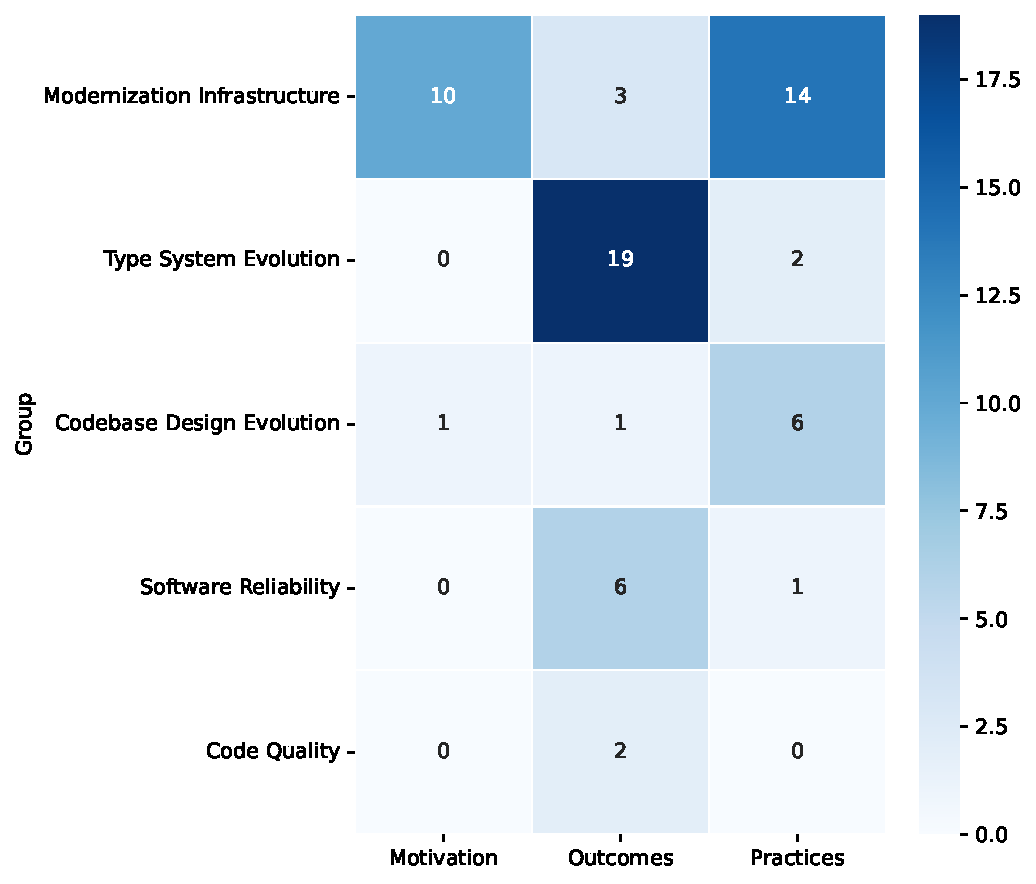
\includegraphics[width=\columnwidth]{imgs/artifacts_ta.pdf}
    \caption{Themes identified from repository artifacts analysis.}
    
    \label{fig:motivation_distribution_artifacts}
\end{figure}

\subsection{Triangulation Results}

\begin{figure*}[!t]
    \centering
    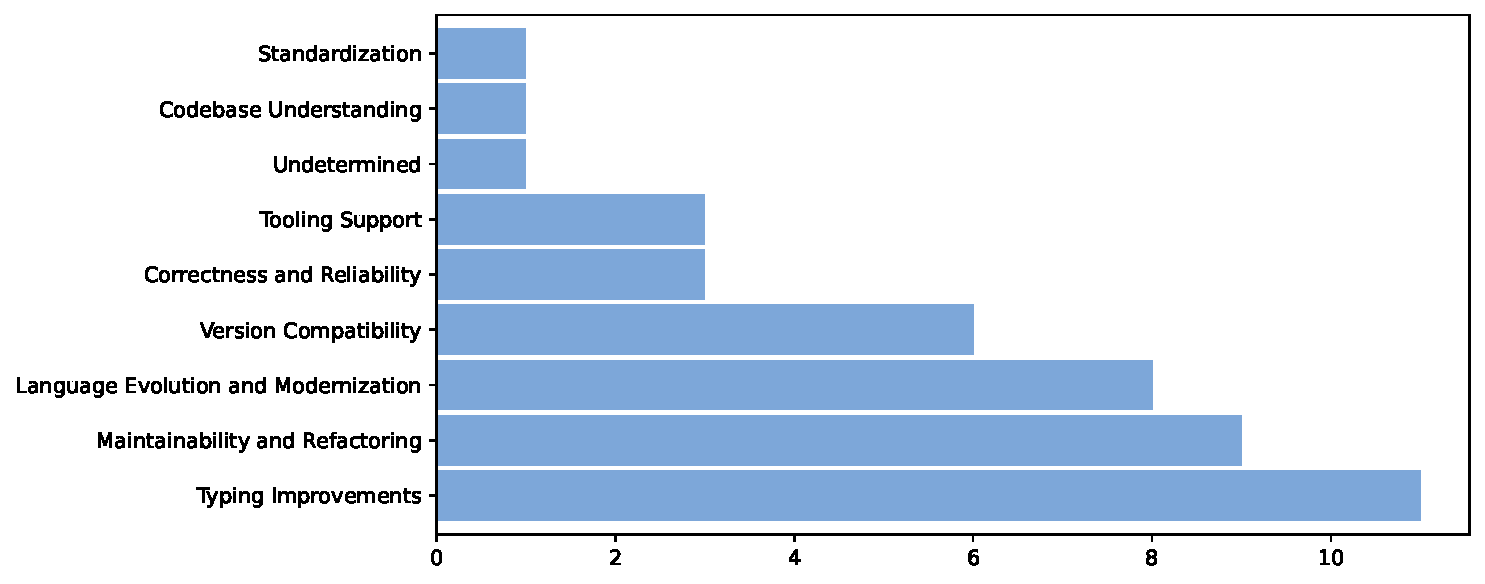
\includegraphics[width=\textwidth]{imgs/triangulation.pdf}
    \caption{Frequency of motivation categories identified across the triangulated cases.}
    \label{fig:triangulation}
\end{figure*}

To assess the consistency between available repository artifacts and developers' feedback, we compared the themes identified from commit messages, pull request discussions, and code review comments with those obtained from the survey responses. Overall, the triangulation revealed a high level of agreement between both sources. 85\% of the analyzed cases demonstrated at least partial convergence regarding the motivations behind the modernization effort.

Beyond validating the consistency of the findings, the triangulation also showed that the two sources provide complementary perspectives on the same development activity, as shown in Figure~\ref{fig:triangulation}. Repository artifacts primarily document the technical rationale of the changes, emphasizing modernization campaigns, Python version migrations, tooling adoption, and implementation strategies. In contrast, survey responses more frequently expose the developers' decision-making process, highlighting perceived benefits such as improved readability, maintainability, type safety and code quality. Consequently, both sources differ in the level of abstraction and the aspects they emphasize.

Across the cases, the most recurrent motivation categories were Typing Improvements ($n=11$), Maintainability and Refactoring ($n=9$), Language Evolution and Modernization ($n=8$), and Compatibility ($n=6$). Less frequent themes included Correctness and Reliability ($n=3$), Tooling Support ($n=3$), Standardization ($n=1$), Codebase Understanding ($n=1$), and one case classified as Undetermined. These categories closely match the dominant themes independently identified in both thematic analyses, reinforcing that large-scale type hint modernization is primarily motivated by software quality improvements, adoption of evolving Python language features, and long-term maintenance concerns rather than isolated code changes.

The observed convergence increases confidence that repository artifacts provide a reliable approximation of developers' motivations in large-scale modernization efforts. At the same time, the survey responses reveal contextual information that is rarely documented in commits and pull request discussions, suggesting that combining both sources produces a richer understanding of developer intent than relying on either source alone.

% The analysis of the 20 commit--pull request--email sets revealed a generally high degree of consistency across the three sources. Overall, most cases showed that the intent behind software changes was similarly expressed across commit messages, pull request descriptions, and email responses.

% In a qualitative assessment of consistency, the majority of cases were classified as exhibiting high consistency, where the same underlying motivation or objective could be clearly identified across all three artifacts. A smaller number of cases showed moderate consistency, typically due to differences in the level of detail or emphasis across sources. Only a few cases exhibited low consistency, generally associated with missing or less explicit information in one of the artifacts, rather than direct contradictions.

% Regarding the identified categories, transformations related to language evolution and code modernization were the most prevalent. These changes include, for example, the adoption of new language constructs, updates to syntax in newer Python versions, and the incorporation of features such as \ths. This category reflects the use of newer language functionalities and the continuous updating of coding standards.

% Next, changes aimed at improving type safety stand out, involving the introduction or refinement of type annotations to reduce potential runtime errors. This category is associated with strengthening the type system and the adoption of gradual static typing within the Python ecosystem.

% Categories such as refactoring, compatibility, standardization, and tooling improvements appeared less frequently, suggesting that most transformations are more strongly associated with language ecosystem evolution than with deep structural code reorganizations or infrastructure-level adjustments.

% The comparison across sources also revealed a clear division of roles in documenting software changes. Commits tend to record operational aspects of the implementation, pull requests provide a broader view of the underlying technical objectives of the transformation, and emails often contribute organizational context and decision-making rationale.

% Taken together, these results indicate that the three sources represent complementary levels of expressing change intent, reinforcing the importance of artifact triangulation for a more comprehensive understanding of the motivations associated with software rejuvenation.

% �� Commits (hash curto)
% Tornado
% 113cf79
% FastAPI
% 3da206c
% Deep Agents (LangChain AI)
% d398a1e
% Django CMS
% 1efaa98
% aiohttp
% 35754d4
% CVAT
% 5ddeda3
% AutoGPT (OpenAI ecosystem project)
% e16e69c
% PyTorch Vision
% a095de1
% LlamaIndex
% e157ebb
% Pipecat
% c4dbe92
% Roboflow Supervision
% fd1277f
% Manim Community
% 8773252
% Freqtrade
% f369151
% Reflex
% 25016f5
% Pipenv
% d6dc5a0
% Wagtail
% 80b1ebe
% Locust
% 9341cf9
% Chia Blockchain
% a447734
% mypy
% 6682563
% Scrapy
% 6ecc9e0